
%%%%%%%%%%%%%%%%%%%%%%%%%%%%%%%%%%%%%%%%%
% Masters/Doctoral Thesis 
% LaTeX Template
% Version 2.4 (22/11/16)
%
% This template has been downloaded from:
% http://www.LaTeXTemplates.com
%
% Version 2.x major modifications by:
% Vel (vel@latextemplates.com)
%
% This template is based on a template by:
% Steve Gunn (http://users.ecs.soton.ac.uk/srg/softwaretools/document/templates/)
% Sunil Patel (http://www.sunilpatel.co.uk/thesis-template/)
%
% Template license:
% CC BY-NC-SA 3.0 (http://creativecommons.org/licenses/by-nc-sa/3.0/)
%
%%%%%%%%%%%%%%%%%%%%%%%%%%%%%%%%%%%%%%%%%

%----------------------------------------------------------------------------------------
%	PACKAGES AND OTHER DOCUMENT CONFIGURATIONS
%----------------------------------------------------------------------------------------

\documentclass[
11pt, % The default document font size, options: 10pt, 11pt, 12pt
%oneside, % Two side (alternating margins) for binding by default, uncomment to switch to one side
english, % ngerman for German
singlespacing, % Single line spacing, alternatives: onehalfspacing or doublespacing
%draft, % Uncomment to enable draft mode (no pictures, no links, overfull hboxes indicated)
%nolistspacing, % If the document is onehalfspacing or doublespacing, uncomment this to set spacing in lists to single
%liststotoc, % Uncomment to add the list of figures/tables/etc to the table of contents
%toctotoc, % Uncomment to add the main table of contents to the table of contents
%parskip, % Uncomment to add space between paragraphs
%nohyperref, % Uncomment to not load the hyperref package
headsepline, % Uncomment to get a line under the header
%chapterinoneline, % Uncomment to place the chapter title next to the number on one line
%consistentlayout, % Uncomment to change the layout of the declaration, abstract and acknowledgements pages to match the default layout
]
{MastersDoctoralThesis} % The class file specifying the document structure

\usepackage[utf8]{inputenc} % Required for inputting international characters
\usepackage[T1]{fontenc} % Output font encoding for international characters

\usepackage{palatino} % Use the Palatino font by default

\usepackage[backend=bibtex,style=numeric,natbib=true]{biblatex} % Use the bibtex backend with the authoryear citation style (which resembles APA)

\addbibresource{example.bib} % The filename of the bibliography

\usepackage[autostyle=true]{csquotes} % Required to generate language-dependent quotes in the bibliography

\usepackage{titlesec} % To add paragraph

\usepackage{mathtools}

\usepackage{lipsum}

\newlength\Colsep
\setlength\Colsep{10pt}

\usepackage{todonotes}

\usepackage{amssymb}
\usepackage{amsmath}
\usepackage{algorithm}
\usepackage[noend]{algpseudocode}

\def \mathbi#1{\textbf{\em #1}}

\makeatletter
\newsavebox\myboxA
\newsavebox\myboxB
\newlength\mylenA

\newcommand*\xoverline[2][0.75]{%
    \sbox{\myboxA}{$\m@th#2$}%
    \setbox\myboxB\null% Phantom box
    \ht\myboxB=\ht\myboxA%
    \dp\myboxB=\dp\myboxA%
    \wd\myboxB=#1\wd\myboxA% Scale phantom
    \sbox\myboxB{$\m@th\overline{\copy\myboxB}$}%  Overlined phantom
    \setlength\mylenA{\the\wd\myboxA}%   calc width diff
    \addtolength\mylenA{-\the\wd\myboxB}%
    \ifdim\wd\myboxB<\wd\myboxA%
       \rlap{\hskip 0.5\mylenA\usebox\myboxB}{\usebox\myboxA}%
    \else
        \hskip -0.5\mylenA\rlap{\usebox\myboxA}{\hskip 0.5\mylenA\usebox\myboxB}%
    \fi}
\makeatother

\DeclarePairedDelimiter\ceil{\lceil}{\rceil}
\DeclarePairedDelimiter\floor{\lfloor}{\rfloor}

\algnewcommand\algorithmicforeach{\textbf{for each}}
\algdef{S}[FOR]{ForEach}[1]{\algorithmicforeach\ #1\ \algorithmicdo}

%----------------------------------------------------------------------------------------
%	MARGIN SETTINGS
%----------------------------------------------------------------------------------------

\geometry{
	paper=a4paper, % Change to letterpaper for US letter
	inner=2.5cm, % Inner margin
	outer=3.8cm, % Outer margin
	bindingoffset=.5cm, % Binding offset
	top=1.5cm, % Top margin
	bottom=1.5cm, % Bottom margin
	%showframe, % Uncomment to show how the type block is set on the page
}

%----------------------------------------------------------------------------------------
%	THESIS INFORMATION
%----------------------------------------------------------------------------------------

\thesistitle{Applying Content-Boosted Collaborative Filtering On Spotify Dataset} 

\supervisor{Prof Anna Monreale} % \supname

\examiner{} % \examname
\degree{Master thesis} % \degreename
\author{Khoi Hoang \textsc{Nguyen}} % \authorname

\addresses{} % Your address, this is not currently used anywhere in the template, print it elsewhere with \addressname

\subject{} % Your subject area, this is not currently used anywhere in the template, print it elsewhere with \subjectname

\keywords{} % Keywords for your thesis, this is not currently used anywhere in the template, print it elsewhere with \keywordnames

\university{\href{http://www.university.com}{Sant'Anna}} % Your university's name and URL, this is used in the title page and abstract, print it elsewhere with \univname

\department{\href{http://department.university.com}{Management Department}} % Your department's name and URL, this is used in the title page and abstract, print it elsewhere with \deptname

\group{\href{http://researchgroup.university.com}{Research Group Name}} % Your research group's name and URL, this is used in the title page, print it elsewhere with \groupname

\faculty{\href{http://faculty.university.com}{Faculty Name}} % Your faculty's name and URL, this is used in the title page and abstract, print it elsewhere with \facname

\AtBeginDocument{
\hypersetup{pdftitle=\ttitle} % Set the PDF's title to your title
\hypersetup{pdfauthor=\authorname} % Set the PDF's author to your name
\hypersetup{pdfkeywords=\keywordnames} % Set the PDF's keywords to your keywords
}

\begin{document}

\frontmatter % Use roman page numbering style (i, ii, iii, iv...) for the pre-content pages

\pagestyle{plain} % Default to the plain heading style until the thesis style is called for the body content


%----------------------------------------------------------------------------------------
%	TITLE PAGE
%----------------------------------------------------------------------------------------

\begin{titlepage}
\begin{center}

\vspace*{.06\textheight}
{\scshape\LARGE \univname\par}\vspace{1.5cm} % University name
\textsc{\Large Master Thesis}\\[0.5cm] % Thesis type

\HRule \\[0.4cm] % Horizontal line
{\huge \bfseries \ttitle\par}\vspace{0.4cm} % Thesis title
\HRule \\[1.5cm] % Horizontal line
 
\begin{minipage}[t]{0.4\textwidth}
\begin{flushleft} \large
\emph{Author:}\\
\href{http://www.johnsmith.com}{\authorname} % Author name - remove the \href bracket to remove the link
\end{flushleft}
\end{minipage}
\begin{minipage}[t]{0.4\textwidth}
\begin{flushright} \large
\emph{Supervisor:} \\
\href{http://www.jamessmith.com}{\supname} % Supervisor name - remove the \href bracket to remove the link  
\end{flushright}
\end{minipage}\\[3cm]
 
\vfill

\large \textit{A thesis submitted in fulfillment of the requirements\\ for the degree of \degreename}\\[0.3cm] % University requirement text
\textit{in the}\\[0.4cm]
\groupname\\\deptname\\[2cm] % Research group name and department name
 
\vfill

{\large \today}\\[4cm] % Date
%\includegraphics{Logo} % University/department logo - uncomment to place it
 
\vfill
\end{center}
\end{titlepage}

%----------------------------------------------------------------------------------------
%	DECLARATION PAGE
%----------------------------------------------------------------------------------------

\begin{declaration}
\addchaptertocentry{\authorshipname} % Add the declaration to the table of contents
\noindent I, \authorname, declare that this thesis titled, \enquote{\ttitle} and the work presented in it are my own. I confirm that:

\begin{itemize} 
\item This work was done wholly or mainly while in candidature for a research degree at this University.
\item Where any part of this thesis has previously been submitted for a degree or any other qualification at this University or any other institution, this has been clearly stated.
\item Where I have consulted the published work of others, this is always clearly attributed.
\item Where I have quoted from the work of others, the source is always given. With the exception of such quotations, this thesis is entirely my own work.
\item I have acknowledged all main sources of help.
\item Where the thesis is based on work done by myself jointly with others, I have made clear exactly what was done by others and what I have contributed myself.\\
\end{itemize}
 
\noindent Signed:\\
\rule[0.5em]{25em}{0.5pt} % This prints a line for the signature
 
\noindent Date:\\
\rule[0.5em]{25em}{0.5pt} % This prints a line to write the date
\end{declaration}

\cleardoublepage

%----------------------------------------------------------------------------------------
%	QUOTATION PAGE
%----------------------------------------------------------------------------------------

\vspace*{0.2\textheight}

\noindent\enquote{\itshape Thanks to Google, Wiki, Stack Overflow for helping me with this monster}\bigbreak

\hfill Khoi Hoang Nguyen

%----------------------------------------------------------------------------------------
%	ABSTRACT PAGE
%----------------------------------------------------------------------------------------

\begin{abstract}
\addchaptertocentry{\abstractname} % Add the abstract to the table of contents
The Thesis Abstract is written here (and usually kept to just this page). The page is kept centered vertically so can expand into the blank space above the title too\ldots
\end{abstract}

%----------------------------------------------------------------------------------------
%	ACKNOWLEDGEMENTS
%----------------------------------------------------------------------------------------

\begin{acknowledgements}
\addchaptertocentry{\acknowledgementname} % Add the acknowledgements to the table of contents
The acknowledgments and the people to thank go here, don't forget to include your project advisor\ldots
\end{acknowledgements}

%----------------------------------------------------------------------------------------
%	LIST OF CONTENTS/FIGURES/TABLES PAGES
%----------------------------------------------------------------------------------------

\tableofcontents % Prints the main table of contents

\listoffigures % Prints the list of figures

\listoftables % Prints the list of tables

%----------------------------------------------------------------------------------------
%	ABBREVIATIONS
%----------------------------------------------------------------------------------------

%\begin{abbreviations}{ll} % Include a list of abbreviations (a table of two columns)

%\textbf{LAH} & \textbf{L}ist \textbf{A}bbreviations \textbf{H}ere\\
%\textbf{WSF} & \textbf{W}hat (it) \textbf{S}tands \textbf{F}or\\

%\end{abbreviations}

%----------------------------------------------------------------------------------------
%	SYMBOLS
%----------------------------------------------------------------------------------------

%\begin{symbols}{lll} % Include a list of Symbols (a three column table)

%$a$ & distance & \si{\meter} \\
%$P$ & power & \si{\watt} (\si{\joule\per\second}) \\
%Symbol & Name & Unit \\

%\addlinespace % Gap to separate the Roman symbols from the Greek

%$\omega$ & angular frequency & \si{\radian} \\

%\end{symbols}

%----------------------------------------------------------------------------------------
%	DEDICATION
%----------------------------------------------------------------------------------------

%\dedicatory{For/Dedicated to/To my\ldots} 

%----------------------------------------------------------------------------------------
%	THESIS CONTENT - CHAPTERS
%----------------------------------------------------------------------------------------

\mainmatter % Begin numeric (1,2,3...) page numbering

\pagestyle{thesis} % Return the page headers back to the "thesis" style

\setcounter{secnumdepth}{4}

\titleformat{\paragraph}
{\normalfont\normalsize\bfseries}{\theparagraph}{1em}{}
\titlespacing*{\paragraph}
{0pt}{3.25ex plus 1ex minus .2ex}{1.5ex plus .2ex}

% Include the chapters of the thesis as separate files from the Chapters folder
% Uncomment the lines as you write the chapters

% Chapter 1

\chapter{Introduction} % Main chapter title

\label{Chapter1} % For referencing the chapter elsewhere, use \ref{Chapter1} 

%----------------------------------------------------------------------------------------

% Define some commands to keep the formatting separated from the content 
\newcommand{\keyword}[1]{\textbf{#1}}
\newcommand{\tabhead}[1]{\textbf{#1}}
\newcommand{\code}[1]{\texttt{#1}}
\newcommand{\file}[1]{\texttt{\bfseries#1}}
\newcommand{\option}[1]{\texttt{\itshape#1}}

%----------------------------------------------------------------------------------------

\section{A statement of the problem}
Recommender system has been an interesting subject of research for long. The idea of recommender system began in early 1990s - with the popularization of the internet, to utilize the critique of millions of people online to help us acquire more useful and interesting content. The PARC Tapestry system \cite{goldberg1992using} first introduced the novel idea of collaborative filtering technique in 1992, which instantaneously became a subject of interest for many other research groups and was employed in many systems, including the GroupLens system \cite{resnick1994open}, the Ringo system at MIT \cite{shardanand1995social}, and the Bellcore Video Recommender \cite{hill1995recommending}.

%----------------------------------------------------------------------------------------



% Chapter 2

\chapter{Background information} % Main chapter title
\label{Chapter2} 

%----------------------------------------------------------------------------------------


%----------------------------------------------------------------------------------------

In this chapter, I will firstly make a survey of different types of recommender systems; then I will narrow down the topic to music recommender systems. As music possess different features comparing to other kind of information such as movie and news, its recommender system also needs to be tailor to bring satisfaction to its listeners.

\section{Overview of recommender systems}
There are currently three main basic approach to recommendation, namely collaborative recommendation, content-based recommendation, and knowledge-based recommendation \cite{jannach2010recommender}. There are also an approach, called hybrid approaches, that tries to combine different recommendation together, in order to augment the strength and limit the drawback of each separate techniques. The description, as well as the advantages and disadvantages, of each recommendation techniques will be discussed as follow.

\subsection{Collaborative recommendation}
The main idea of collaborative recommendation approaches is to predict potential items that a user would like using past behavior information of other users. Pure collaborative algorithm take only user-item ratings as input and generate a prediction suggesting to what degree the user will like a certain item or a list of \textit{n} recommended items as output. 

There are two kind of ratings that can be used, namely implicit and explicit ratings. Explicit rating information can be collected by explicitly asking users to rate the item on a specific scale. Different scales are applied to different domain, as the quality of recommendation is different between these scales \cite{cosley2003seeing}. Ratings are then convert internally to numeric values in order for recommender systems to calculate the similarities. Implicit ratings, on the other hand, are knowledge collected based on the interaction between users and the systems. They can be in various forms with distinctive characteristics, such as information about item buying, book reading, music listening, or even user browsing behavior. As implicit ratings are observed behaviors, recommenders have to interpret whether the behaviors have positive or negative impacts toward the users. Even though the interpretation might be incorrect in some cases (e.g., a user might not like all the items that she bought), a massive amount of feedback would exclude these particular cases. In fact, Shafer et al \cite{schafer2006recommender} report that in some domains, user model using implicit information can outperform the one with explicit ratings.

There are many algorithms develop to exploit the rating matrix; However, in this review, I will just go into detail some main approaches that have been studied carefully in the past and have been applied widely in the industry. These approaches include user-based approach, item-based approach, and an approach using matrix factorization/ latent factor models. Some other approaches, such as probabilistic approach, or slope one predictors, will not be mentioned here because of the scope of the thesis.

\subsubsection{User-based nearest neighbor recommendation}
\textit{User-based nearest neighbor recommendation} is one of the earliest algorithm for this approach. The main idea of the algorithm is to identify other users who have similar preferences to a user; then for any item \textit{i} that is unknown to the current user, a prediction is given based on the similar of the ratings of other users on item \textit{i}.

\paragraph{Pearson's correlation coefficient}
One common method to calculate the similar between users is Pearson's correlation coefficient. The general formula for the coefficient \(\rho\) \cite{benesty2009pearson} is:

\begin{displaymath}
\rho_{X,Y} = \frac{cov(X,Y)}{\sigma_X \sigma_Y}
\end{displaymath}

with \(cov(X,Y)\) is the covariance between X and Y, and \(\sigma_X\) and \(\sigma_Y\) represent the standard deviation of X and Y. 

Apply the formula to the case of collaborative filtering: let \( $\mathbf{U}$ = \{ $\mathbf{u_1}$, \dots, $\mathbf{u_n}$\} \) denote the set of users, \( $\mathbf{U}$ = \{ $\mathbf{p_1}$, \dots, $\mathbf{p_n}$ \}$ \) for the set of items. The 2 sets form a \(n \times m\) matrix of rating \(r_{i,j}\) with \(i \in 1 \dots n, j \in 1 \dots m\), with \(r_{a,p} \) is the rating of user a on item p, and \(\bar{r}_a \) denotes the average rating of user a. The similarity of user a and b \(sim(a, b) \) is defined as follow:

\begin{displaymath}
sim(a,b) = \frac{\sum_{p \in P}(r_{a,p} - \bar{r}_a)(r_{b,p} - \bar{r}_b)}{\sqrt{\sum_{p \in P}(r_{a,p} - \bar{r}_a)^2} \sqrt{\sum{p \in P}(r_{b,p} - \bar{r}_b)^2}}
\end{displaymath}

The Pearson correlation coefficient takes value range from -1 to +1, indicating respectively from a strong negative correlation to a strong positive correlation.

\paragraph{Other weighting metrics}
Apart from Pearson's correlation coefficient, other metrics, such as adjusted cosine similarity, Spearman's rank correlation coefficient, or mean squared difference measure are also proposed to calculate user-based similarity. However, empirical study made by Herlocker et al \cite{herlocker1999algorithmic} shows that for user-based recommender system, the Pearson coefficient outperforms other measures.

Still, the "pure" Pearson measure alone is not ideal as there are cases that the measure cannot handle. Consider a real life problem that there are some items that are favored by everyone, Pearson's measure would not consider that an agreement by two users on a controversial item has more weight than an agreement on a universally like item. Herlocker et al \cite{herlocker1999algorithmic} also showed that applying the measure to user who has rated very few items also lead to bad predictions. Therefore, many attempts, such as significance weighting proposed by Herlocker et al \cite{herlocker1999algorithmic}, or case amplification suggested by Breese et al \cite{breese1998empirical} have been made to fill the gap and improve the accuracy. However, the question of whether these weighting schemes are helpful in real-world settings is still opened.

\paragraph{Challenges}
Although user-based approaches have been deployed successfully, they faces serious challenges when are applied to large e-commerce sites which possess millions of users and items. Specifically, the cost for scanning a vast number of potential neighbors makes it impossible for the system to predict in real time. Therefore, large scale e-commerce sites often opt for other techniques, one of them is the item-based nearest neighbor approach.

\subsubsection{Item-based nearest neighbor recommendation}
The main idea of this approach is to calculate the similarity between items instead of one between users. The advantage of this approach over user-based approach is that we can preprocess an item similarity matrix that characterize the degree of similarity between items. At run time, a prediction for product p and user u is made by detecting the most relevant items using the item similar matrix and by calculating the weighted sum of u's rating for these items. As the number of relevant items is commonly limited, the computation of the prediction can be done within a short time frame, suitable for such online applications. A similar matrix is, theoretically, also possible with user-based approaches; however, in real time scenarios, the number of overlapping ratings for two random users is relatively small, making it unstable as a few more ratings may significantly affect the similarity between users.

For item-based approaches, the cosine similarity is found to be the standard metric \cite{jannach2010recommender}. The cosine similarity is defined as follows:

\begin{displaymath}
sim(\overrightarrow{a}, \overrightarrow{b}) = \frac{\overrightarrow{a} \cdot \overrightarrow{b}}{|\overrightarrow{a}| * | \overrightarrow{b} |}
\end{displaymath}

where \( \overrightarrow{a} \) is an item vector, \( \cdot \) denotes the dot product, and \(|\overrightarrow{a}| \) is the Euclidian length of the vector, which is defined as the square root of the dot product of the vector with itself. 

One drawback of cosine measure is that it does not take into account the fact that different users have different rating schemes, i.e., some users rate items highly in general, while some others give lower ratings. This drawback is solved using adjusted cosine measure, which subtracts the user average from the rating. Let \( U\) be the set of users that rate both item \(a\) and \(b\). The adjusted cosine measure is as follows:

\begin{displaymath}
sim(a,b) = \frac{\sum_{u \in U}(r_{u,a} - \bar{r}_u)(r_{u,b} - \bar{r}_u)}{\sqrt{\sum_{u \in U}(r_{u,a} - \bar{r}_u)^2} \sqrt{\sum{u \in U}(r_{u,b} - \bar{r}_u)^2}}
\end{displaymath}

with \(\bar{r}_u \) is the average rating for item u.

The prediction function, which is computed in real time, is defined as follows:

\begin{displaymath}
pred(u,p) = \frac{\sum_{i \in ratedItem(u)}{sim(i,p) * r_{u,i}}}{\sum_{i \in ratedItem(a)}{sim(i,p)}}
\end{displaymath}

Compare to user-based recommendation, item-based approaches prove to be often more scalable as for most of the case, the number of items falls behind the number of user, thus it requires less time and space to compute the similarity matrix (if necessary). Also, item-based approaches are more justifiable by users, for they can easily grasp the explanation of the recommendation, modify the list of neighbors and alter the weights. User-based methods, on the other hand, are less able to justify, as recommendations come from other users are hard to explain. However, as item-based approaches are based on ratings on similar items, the recommender tend to suggest items that might be already familiar to that user. While this behavior leads to safe recommendations, it does not help users explore other novel items that they might like as well.

In general, nearest neighbor approaches work well for popular items. Nonetheless, there are two important drawbacks with these approaches when deal with unpopular item:

\begin{itemize}
\item[•] Limited coverage: both approaches define neighbor as having ratings in common. This assumption is limiting, as users with very few common items can still have similar preferences. Moreover, coverage of such approaches can be limited, as only items rated by neighbor can be recommended.

\item[•] Sensitive to sparse data: For most system, users only rated a small portions of available items. This results in a cold star problem, when some items have very few or no ratings at all, which affects the prediction of these items. Another problem is when there are only few ratings, the weight of each item has a significant impact over the similarity between vectors, reducing the accuracy of the recommender. 
\end{itemize}

To solve these problem, many small tunes for the neighborhood approaches have been made, such as the use of Significance Weighting \cite{} for the weighting problem or ... for the Cold Start problem \cite{}. Besides that, other advance algorithms have also been developed to tackle these topics. One of the most popular approach that has gained attraction recently is the use of matrix factorization, as it was exploited to significantly improve the accuracy of the recommender system in the Netflix Prize competition in 2009.

\subsubsection{Matrix factorization/ latent factor model}
Matrix factorization methods is used to derive a set of salient patterns from user-ratings. For example, let "Gone with the wind" and "Me before you" be the set of liked item of user A, and "Romeo and Juliet" and "The fault in our star" be the set of liked item of user B, while nearest neighbor approaches would consider these books separately, matrix factorization could see that all these books belong to romantic genre and therefore recommend them to the other user. The factors, however, is not always obvious. In some cases, they can be uninterpretable.

The idea of this method is to factorize the original sparse matrix into a product of matrices. Each decomposed matrix is much denser than the original one. The technique can be used for both similarity matrix and rating matrix. There are many matrix factorization techniques with increasing complexity and accuracy. For the scope of this thesis, I will demonstrate Singular value decomposition (SVD) model, a basic yet effective decomposition technique. The example is an adaptation from the one from Grigorik \cite{I. Grigorik}. 

Consider the table 2.1:

\begin{table}
\centering
\begin{tabular}{c c c c c}
\hline\hline
& User 1 & User 2 & User 3 & User 4 \\
\hline
Item 1 & 3 & 4 & 3 & 1 \\
Item 2 & 1 & 3 & 2 & 6 \\
Item 3 & 2 & 4 & 1 & 5 \\
Item 4 & 3 & 3 & 5 & 2 \\

\hline\hline \\
\end{tabular}
\caption{Rating for SVD-based recommendation}
\label{table:1}
\end{table}

SVD takes a m-by-n matrix M and decomposes it into three factors: two unitary matrices U and V, and a nonnegative diagonal matrix \(\Sigma \). The main point of this decomposition is that after receiving the product matrix, we can retain only  The decomposition is as follows:

\begin{displaymath}
M = U \Sigma V^T
\end{displaymath}

where \(V^T\) is the transpose matrix of V. 

Applying the decomposition, we obtain \(\Sigma = {12.2215, 4.9282, 2.0638, 0.2977} \) and the two matrices

\noindent\begin{minipage}[t]{\textwidth}
\begin{minipage}[c][5cm][c]{\dimexpr0.5\textwidth-0.5\Colsep\relax}

\begin{tabular}{c c c c}
\hline\hline \\
U \\
\hline \\
-0.4312 & 0.4932 & -0.5508 & -0.5172 \\
-0.5327 & -0.5305 & 0.4197 & -0.5085 \\
-0.5237 & -0.4052 & -0.4873 & 0.5693 \\
-0.5059 & 0.5578 & 0.5321 & 0.3871 \\
\hline\hline
\end{tabular}

\end{minipage}\hfill
\begin{minipage}[c][5cm][c]{\dimexpr0.5\textwidth-0.5\Colsep\relax}

\begin{tabular}{c c c c}
\hline\hline \\
V \\
\hline \\
-0.3593 & 0.3677 & -0.2961 & 0.8050 \\
-0.5675 & 0.0880 & -0.6285 & -0.5246 \\
-0.4429 & 0.5686 & 0.6590 & -0.2150 \\
-0.5939 & -0.7306 & 0.2882 & 0.1746 \\
\hline\hline \\
\end{tabular}
\end{minipage}%
\end{minipage}



\section{Overview of music recommender systems}
Music, differs from other content domains such as books or movies, has its own unique characteristics regarding consumption. For example, the consumption time of books and movies are quite lengthy, ranging on the average of few hours (for movies) to several days (for books); songs, on the other hand, takes a much shorter time for listener to consume, only a few minutes. Consequently, this lead to the ephemeral and disposable nature of music. Another example is the number of repetition: a single song can be consumed repeatedly (even multiple times in a row), while books are movies are consumed a few times at most. This implies that the user might appreciate recommendations of items that they already heard in the past.

In the past, many approaches, based on the observation of the nature of music and listener's behaviors, had been tried to build an efficient music recommender system. Till now, there are three main approaches to such system \cite{ricci2011introduction}, which will be described in the following sections. 

\subsection{Content-Based Music Recommendation}

Content-based recommendation exploits information describing music as material for recommender systems. There are two main approaches for content-based system: one uses metadata, such as annotations or social tags, while the other analyses audio content using machine learning techniques.

\subsubsection{Metadata content}
Metadata comes in several forms. One is the manual annotations constructed by music experts or voluntary community. This kind of annotation often obeys a strict structured taxonomy build by expects. Another form of annotations is social tags, which is built by asking casual users to provide unstructured text annotations for the item. The last kind of annotations is information collected on web pages, blogs and RSS feeds related to music items.

\paragraph{Annotation} 
Manual annotation contain information such as musical genre, record label, year, knowledge about tracks and artists, and albums. Some musical properties, particularly tempo, mood, and instrumentation can also be added. Many online database have been built using editorial metadata, following by many recommender systems trying to exploit them. 

Bogdanov et al. \cite{bogdanov2012taking} build an artist recommender using exclusively metadata from \textit{Discogs}, a free and community-built database containing information about artists, records labels, and their releases. For each artist in the database, a tag weight vector is created using genre, style, label, country, and year information of the releases related to the artist. The role of the artist in each release (e.g. main artist, track artist, or extra artist) and the relations between artist, such as aliases and membership relations, are also taken into account. A sparse tag matrix is then formed from the artist vectors, and latent semantic analysis \cite{deerwester1990indexing} is applied to reduce the dimension of the matrix. Afterwards, the authors use Pearson correlation distance \cite{gibbons2011nonparametric} to measure the similarity between artists.

Apart from community-built database, some other database are developed by experts for commercial use. \textit{Pandora}, for example, is a personalized radio that built its recommender using annotations done by experts \cite{jones2007user}. \textit{AllMusic} is another example that also provides mood annotations besides general editorial metadata. However, not much research has been done using these database, as they are proprietary, and there is no public data sets of this kind are available for researcher. Constructing such a data set would be costly, and they are difficult to scale to large collections.

\paragraph{Social tags}
Social tags are tags provided by user using the services. Tags are personalized, arbitrary, and do not follow any particular structure, ranging from genre like "blue" or "jazz" to event-related attributes (e.g. "live") and assertion (e.g. "my favorite song"). They also vary in scope, from broad one such as "classical" to niche terminology like "Malcolm Arnold" or "renaissance". Social tags, therefore, need to be preprocess for the data to be useful. A popular method, which is used by \textit{Last.fm}, a social music website, for structuring social tags is to transform them into a folksonomy \cite{sordo2008quest}. The tag weight vectors technique is then applied to compute the similarity \cite{green2009generating}, with the enhancement by using latent semantic analysis techniques to overcome vector sparsity problem \cite{levy2008learning}

\paragraph{Annotations by web crawling}
Apart from tags made by experts and social tags, some recommender systems are built using information crawled from web pages. These recommenders often apply artist similarity metric, generated by using text mining techniques \cite{schedl2011exploring}, as the main principle for the recommendation. Green et al. \cite{green2009generating} compute artist-to-artist similarity using keyword extracted from \textit{Wikipedia} entries and social tags from \textit{Last.fm}. Similarly, McFee and Lanckriet \cite{mcfee2011learning} predict artist similarity based on social tags and keyword extracted from artist biographies on \textit{Last.fm}. A deviant approach is the one made by Lim et al., as they compute song-level similarity through bag-of-words representations of lyrics found on \textit{musiXmatch.com} \cite{lim2013robust}

\subsubsection{Audio content}
Audio content analysis is promoted by MIR researchers as an alternative to metadata and collaborative filtering method \cite{barrington2009smarter}. Content analysis is expected to solve "long tail" problem, where unpopular music items are not suggested because the lack of available user ratings, tags, and other types of metadata \cite{celma2009music}. Music content is separated into two broad categories: acoustic features taken directly from the audio, and semantic annotations derived from acoustic features using machine learning techniques. 

\paragraph{Acoustic features}
Acoustic features are properties 	of a sound that can be recorded and analyzed using signal processing techniques. There are three kinds of features that are used by recommender system:

\begin{itemize}
\item[•] Timbral features: features related to spectral content (i.e. shape) of the signal;
\item[•] Temporal and time-domain features: features such as loudness, tempo, onset rate;
\item[•] Tonal features: musical component such as harmonic pitch, key, scale, and chords distribution.
\end{itemize}

Timbral similarity method converts timbre information to a standard representation and applies a number of methods to approximate the likelihood between two songs \cite{aucouturier2005way} \cite{logan2001music}. For example, Logan \cite{logan2004music} builds a recommender that compares Mel-frequency cepstrum coefficient (MFCC) based distance of user's music set with target play list. The approach, however, is insufficient as evaluation shows a nominal number of customer satisfaction \cite{bogdanov2013semantic}. 

Pampalk et al. \cite{pampalk2005improvements} \cite{pampalk2005dynamic} study an algorithm that use, in addition to spectral similarity, loudness fluctuations and two derived descriptors from sound wave to improve the accuracy of music similarity and genre classification of a song. The algorithm is used to recommend user playlists, in which songs that are similar to the ones that are skipped by user are eliminate, and only tracks that are similar to the ones that the user wholly listens to remains.

Celma and Herrera \cite{celma2008new} take another approach, calculating Euclidean distance using timbre, dynamics, tempo, meter, tonal strength, key, and mode information. This method is compared to an item-based collaborative filtering and a hybrid method on a large scale evaluation. The result shows that all three algorithms work fine recommending familiar items. For unfamiliar items, collaborative filtering reveals a poor discovery ratio, while pure content-based method sometimes goes off direction (it is technically difficult to differentiate between the sound of classical guitar and the one of harpsichord). The hybrid method performs the best, as it limit the number of possible tracks whose artists are related with the original artist, therefore reducing mistakes performing by pure content-based method.

\paragraph{Semantic annotation}
Pure acoustic signal, unfortunately, cannot directly capture semantic meaning of a track. As a result, mere acoustic feature recommenders do a poor job in song suggestion, as an "energetic" song can be recommended next to a "nostalgic" track because of the similarity of the instrument. A sudden change in genre might frustrate customer, as one would not expect a mourning song in a middle of a party. Therefore, many approaches have been made in order to bridge this semantic gap by using machine learning techniques to predict annotations from audio content.

However, extracting genre or mood information from acoustic content is perplexing, as mapping between human annotation and acoustic cannot be clearly defined \cite{aucouturier2009sounds}. To solve this,  Barrington et al. \cite{barrington2009smarter} propose a method to measure semantic similarity: they train Gaussian mixture models of MFCCs for semantic concepts such as genres, moods and instruments. Therefore, for a song, a distribution of tags is generated, which is then compared to another in order to estimate similarity. 

\subsection{Contextual Music Recommendation}
The vast majority of existing recommender system approaches focus on information about users and items but not context information, such as time and place of the event. Only until recently, the topic of context-awareness starts to gain attraction in recommender system research \cite{adomavicius2011context}. Context, in the fields that are directly related to recommender system, is defined as "information describing where you are, whom you are with, and what resources are nearby" \cite{schilit1994context}. Therefore, context in the domain of music can be derived as a collection of factors that affects user's appreciation of music, such as time, mood, and current activities.

Contextual information can be classified using various kind of classifications. Adomavicius et al. \cite{adomavicius2011context} suggest categorizing context into three distinct classes: fully observable, partially observable, and unobservable context. Dey and Abowd \cite{abowd1999towards}, in attempt to construct another classification, propose to classify context into primary context, which is four most important factors that describe user situation: location, identity, activity, and time; and secondary context, which is data derived from primary information. Applying the classification of Dey and Abowd, M. Schedl et al \cite{schedl2015music} divide context information into two generic classes: environment-related context and user-related context. Environment-related context refers to information that can be obtained by user's computer or mobile phone, such as location, time, weather, etc., while user-related context indicates information that can be derived from the environment-related one, such as user's activity, emotion state, and social environment. 

\subsubsection{Environment-Related Context}
Surrounding environment has been proven to have an influence on user's preference of music. Adrian C. North and David J. Hargreaves \cite{north1996situational} find a correlation between musical descriptors, such as arousal, sensuality, spirituality, and listening situation, such as activity, spirituality, and social constraint. Pettijohn et al. \cite{pettijohn2010music} find that different seasons, such as winter and summer, also affect musical preferences. 

Many attempts have been made to build recommender using environment-related information. Reddy and Mascia \cite{reddy2006lifetrak} used space information capturing using GPS coordinates, internal time data, kinetic information derived from difference in GPS signals, and even meteorological info to build a recommender for a mobile music player called Lifetrak. Songs have to be tagged manually by users using system predefined tagging system, and are played in appropriate situation based on users' preferences. For example, the app may play rock music when a user is in a gym, and classical music when the user tries to study in a cafeteria. 

Ankolekar and Sandholm from HP labs \cite{ankolekar2011foxtrot} propose a mobile audio application, Foxtrot, that exploits crowd-sourced geo-tagged audio information to provide a stream of location-aware audio content to the users. The recommender, however, generated poor user experiences, as an environment generates different meaning to different people, leading to diverse music preferences. Indeed, a research made by Okada et al. \cite{okada2013contextplayer} shows that not only the algorithm, but also the architectural design and usability of the application that matter, as user feedback suggests the need for explanations of the recommendations and more control over the playlist. 

\subsubsection{User-Related Context}
One's music preference is not only affected by geological and activity component, but also by factors such as emotions and social background. Sch{\"a}fer and Sedlmeier \cite{schafer2009functions} discovered that one's music preference is also linked with one's sociocultural and physiological functions. In other words, people use music preference as a mean to express their identities and personal values. User-related context can be divided into the following groups:

\begin{itemize}
\item[•] Activity information: information implies user's actions (e.g., walking, driving, working) or user's state (e.g., walking pace or heart rate). Foley \cite{foley1940occupational} showed that people with different occupation have different favored music tempo. For example, those who work with power machines like a slow allegro, while typists prefer faster tempo like presto. 
\item[•] Emotional information: current mood of user has a direct impact on the choice of music. For example, a user may want to listening energetic music while he is happy, and calm music vice versa. Sch{\"a}fer and Sedlmeier \cite{schafer2009functions} found that music has a function to moderate listener's mood by energizing him or making he feel better.
\item[•] Social context information: music preference can be affected by the presence of other people. People may choose music taken into account the event they participate in. Many researchers have address the issue of group recommender system. For example, Popescu and Pu \cite{popescu2011probabilistic} proposed using probabilistic weighted sum as the algorithm to recommend group playlist.
\item[•] Cultural context information: information about user's culture characteristics. Koenigstein et al. \cite{koenigstein2009predicting} exploited file sharing information on a Peer to Peer network in US to predict the success of a song on Billboard Hot 100 Chart. Schedl \cite{schedl2013leveraging} built a location-aware recommender system by retrieving geo-tagged Twitter tweets to detect listening trend at a particular place. 
\end{itemize}

Compare to environment-related context, user-related context is more difficult to infer using electronic devices. Many attempts have been made to predict user's emotion or daily activities \cite{park2006context} \cite{wang2012context} by extracting environment-related feature such as the time of day, temperature, weather, etc... Emotion-based music recommender has gained attention recently, due to advances in automatic music emotion recognition \cite{yang2012machine}




 
\chapter{Implementation} % Main chapter title

\label{Chapter3} % For referencing the chapter elsewhere, use \ref{Chapter1} 

In this chapter, the approaches used in this research is examined. First, the dataset taken from Spotify is mentioned. After that, the three algorithms and the evaluation metrics are discussed in detail.

\section{Dataset}

The dataset for this thesis is a combination between two databases from two services: last.fm \footnote{https://last.fm} and Spotify Web Api \footnote{https://developer.spotify.com/web-api}. First, a list of user, the album they listen, the artists, and the number of times they listen to the album is taken from last.fm. The album name and artist name are then used to get album tracks, which are all the tracks contain in that album, on Spotify. Finally, using the track id of each tracks, track audio features are crawled. Then, for each album, the mean of the acoustic features is calculated, which represents the acoustic features of the whole album. The ultimate dataset, creating by joining the mention above databases, contains the following fields:

\begin{itemize}
\item[•] Username: The user who listen to the album, taken from last.fm database.
\item[•] Album: The name of the album the user listens to.
\item[•] Artist: The artist who performs the album.
\item[•] Playcount: The total number of time the user listens to the album.
\item[•] Energy: A perceptual measurement of intensity and activity in a range from 0 to 1. The higher the score, the higher the energy the track contains. For example, metal rock has high energy, while a Bach prelude is perceived to have low energy. This measurement is built on top of dynamic range, loudness, timbral, onset rate, and general entropy.
\item[•] Speechiness: A measurement of how much spoken words is present compare to music. A value from 0.66 to 1 indicates that the track is mostly spoken words, such as talk show or audio book. Vice versa, a value between 0.33 and 0.66 implies that the track contains both music and speech, ranging from pop to rap music. A value below 0.33 indicates a non speech track. 
\item[•] Acousticness: A evaluation of how much acoustic a track contains compare to how much electronic. Again, a value closer to 1 implements that the track is played with mostly acoustic instruments, such as guitar and harmonica; while a value closer to 0 implements the present of electronic instruments.
\item[•] Danceability: A measurement of how suitable a track is for dancing based on a combination of musical elements including tempo, rhythm stability,  beat strength, and overall regularity. The higher the value, the more danceable the track.
\item[•] Tempo: The overall estimated tempo of a track, measuring in beats per minute (BPM).
\item[•] Instrumentalness: The assessment of how much a track incorporates vocals. The higher the instrumentalness, the greater likelihood the track contains no vocal content. 
\item[•] Key: The key (tonal center) a track is in. Integers map to pitches using Pitch Class notation \footnote{https://en.wikipedia.org/wiki/Pitch_class}. 
\item[•] Duration\_ms: The duration of a track in milliseconds.
\item[•] Valence: A measure from 0 to 1 of the positiveness of a track. Tracks with high valence sound more positive (e.g. happy, cheerful), and vice versa.
\item[•] Liveness: An indication of whether a track is performed live or in studio. The higher the liveness, the higher possibility that the track is performed live.
\item[•] Loudness: The overall loudness of a track in decibels (dB), with range from -60 to 0 db. 
\end{itemize}

As some of the features (e.g. key, duration) are not in the scale from 0 to 1, a standardization is necessary to eliminate over-weighting variables. The standardization for all the acoustic features is achieve by subtracting the mean following by dividing by the standard deviation for each feature. 

\todo{add correlation part}

\section{Algorithms}

The following sections describe my implementation of the three algorithms: a pure collaborative filtering, a pure content-based filtering, followed by the details of the hybrid approach.

\subsection{Pure Collaborative Filtering}
As the number of song outnumbers the number of user, I decide to implement the user-user based collaborative filtering. The algorithm can be summarized in the following steps:

\begin{enumerate}
	\item Calculate similarity between users as Pearson correlation between users' rating vectors. 
	\item For each user, form a neighborhood of \textit{n} users that have the highest similarity.
	\item Compute a prediction for an item from a weighted combination of selected neighbor's ratings. 
\end{enumerate}

In step 3, predictions are calculated using \todo{add formula}

\subsection{Pure Content-based Filtering}
The algorithm for pure content-based approach is similar to the one of the pure collaborative filtering. Acoustic features are treated as elements of the item vector for each track. However, one difference is that, instead of using Pearson correlation, the cosine similarity is used for calculating the similarity between items.

\subsection{Content-boosted Collaborative Filtering}
The idea of the content-booasted collaborative filtering algorithm is quite simple. First, a pseudo user-ratings vector is created for every user in the database. Each element of a pseudo user-ratings vector of a user is the user-rating if available, or the value predicted by the content-based recommender otherwise. The formal definition of a pseudo vector is as follow:

\begin{displaymath}

\end{displaymath}

when \( r_(u,i) \) denotes the actual rating of user u for item i, and \(c_(u,i) \) is the prediction of the content-based predictor. 

The pseudo user-ratings vectors of all user together construct a dense pseudo user-rating matrix. This matrix is then used as a substitution of the original user-rating matrix for collaborative filtering method. 






%\chapter{Experimental Evaluation} % Main chapter title

\label{Chapter4}

In this section, the methodology, metrics for the evaluation between different algorithms, as well as the result of the experiment are presented.

\subsection{Methodology}
 
%\chapter{Experimental evaluation} % Main chapter title

\label{Chapter5} % For referencing the chapter elsewhere, use \ref{Chapter5} 

In this section, data exploration, the experimental setup, the metrics for the evaluation between the three algorithms, as well as the result of the experiment are presented.

\section{Data exploration}
\subsection{Descriptive Data Summarization}

In this section, some basic descriptive statistics of the data will be described, in order for the understanding of the overall picture of the data. Figure \ref{fig:boxplot} represent the boxplot diagrams of the energy, speechiness, acousticness, danceability, tempo, instrumentalness, valence, liveness, and loudness respectively. For key, mode, and time signature, as they are categorical variables, boxplot diagram information is not useful. Instead, for these variables, the frequency of the values, such as in table \ref{fig:freq_table} is displayed.

\begin{figure}
  \begin{subfigure}[b]{0.3\textwidth}
    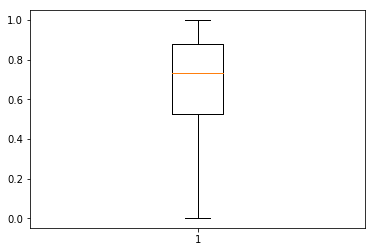
\includegraphics[width=\textwidth]{energy}
    \caption{Energy}
    \label{fig:energy}
  \end{subfigure}
  \hfill
  \begin{subfigure}[b]{0.3\textwidth}
    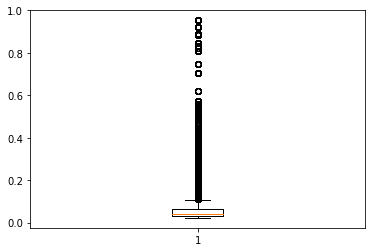
\includegraphics[width=\textwidth]{speechiness}
    \caption{Speechiness}
    \label{fig:speechiness}
  \end{subfigure}
  \hfill
  \begin{subfigure}[b]{0.3\textwidth}
    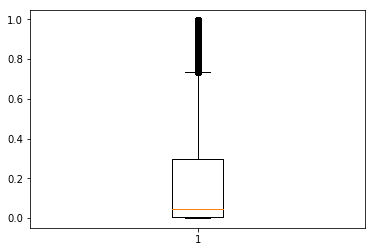
\includegraphics[width=\textwidth]{acousticness}
    \caption{Acousticness}
    \label{fig:acousticness}
  \end{subfigure}
  
  \bigskip
    \begin{subfigure}[b]{0.3\textwidth}
    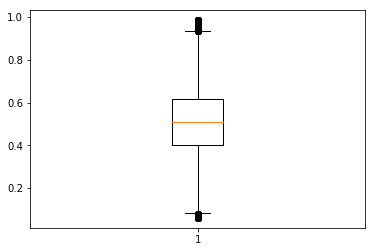
\includegraphics[width=\textwidth]{danceability}
    \caption{Danceability}
    \label{fig:danceability}
  \end{subfigure}
  \hfill
    \begin{subfigure}[b]{0.3\textwidth}
    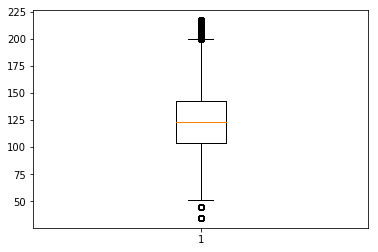
\includegraphics[width=\textwidth]{tempo}
    \caption{Tempo}
    \label{fig:tempo}
  \end{subfigure}
  \hfill
    \begin{subfigure}[b]{0.3\textwidth}
    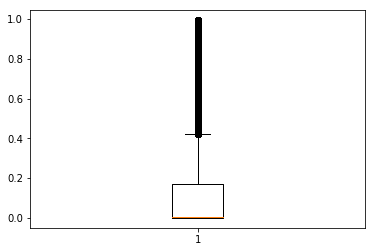
\includegraphics[width=\textwidth]{instrumentalness}
    \caption{Instrumentalness}
    \label{fig:instrumentalness}
  \end{subfigure}
  
  \bigskip
      \begin{subfigure}[b]{0.3\textwidth}
    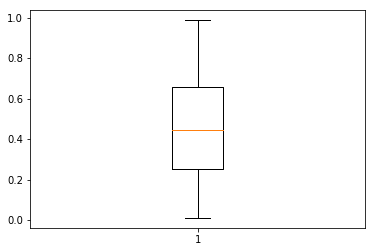
\includegraphics[width=\textwidth]{valence}
    \caption{Valence}
    \label{fig:valence}
  \end{subfigure}
  \hfill
    \begin{subfigure}[b]{0.3\textwidth}
    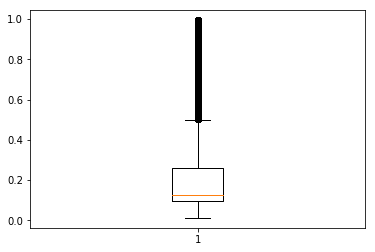
\includegraphics[width=\textwidth]{liveness}
    \caption{Liveness}
    \label{fig:liveness}
  \end{subfigure}
  \hfill
    \begin{subfigure}[b]{0.3\textwidth}
    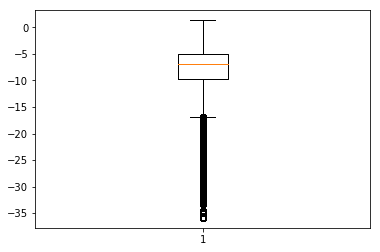
\includegraphics[width=\textwidth]{loudness}
    \caption{Loudness}
    \label{fig:loudness}
  \end{subfigure}
  
  \caption{Boxplot diagram of music features}
  \label{fig:boxplot}
\end{figure}

\begin{figure}
  \begin{subfigure}[b]{0.3\textwidth}
    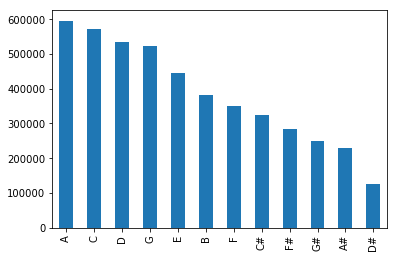
\includegraphics[width=\textwidth]{key}
    \caption{Key}
    \label{fig:key}
  \end{subfigure}
  \hfill
   \begin{subfigure}[b]{0.3\textwidth}
    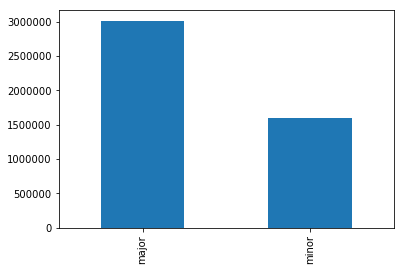
\includegraphics[width=\textwidth]{mode}
    \caption{Mode}
    \label{fig:mode}
  \end{subfigure}
  \hfill
  \begin{subfigure}[b]{0.3\textwidth}
    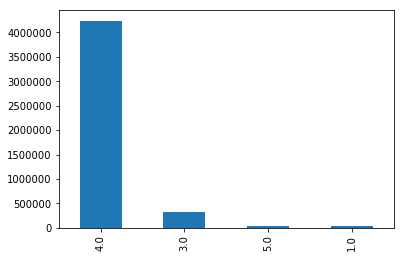
\includegraphics[width=\textwidth]{time_signature}
    \caption{Time signature}
    \label{fig:time_signature}
  \end{subfigure}
	
	\caption{Frequency table of music features}
	\label{fig:freq_table}
\end{figure}

\bigskip

\noindent We can see that from the diagrams:
\begin{itemize}
	\item Energy: the median is quite high, at nearly 0.8. However, the interquartile range of the energy is 0.35, suggesting that the energy spans equally across the value range.
	\item Speechiness: the median is at 0.04, with the first quartile at 0.03 and third quartile at 0.06, showing that most of the tracks have low level of spoken word. 
	\item Acousticness: the median is also at 0.04, with the first quartile at 0.003. However, the third quartile is at 0.3, suggesting that most of the tracks are not acoustic.
	\item Danceability: the median is at 0.5, with the first quartile at 0.4 and third quartile at 0.6, showing a normal distribution, which means that people listen equally to danceable track as well as undanceable track.
	\item Tempo: the median tempo is 123, with the first quartile of 104 and third quartile of 142, suggesting that most people listen to Allegro, which is fast and bright music.
	\item Instrumentalness: the median of 0.003 and the third quartile of 0.17 imply that most of the tracks contain vocal and not just pure instrument.
	\item Valence: with the median of 0.44, first quartile of 0.25, and third quartile of 0.66, valence also forms the normal distribution, suggesting that people listen equally to both positive and negative music.
	\item Liveness: the median of 0.12 and third quartile of 0.25 indicate that most tracks have a low level of liveness.
	\item Loudness: the first quartile of -9 and third quartile of -5 implement that most song have quite the same level of loudness.
	\item Key: songs with different key have different playing frequency. Overall, major key songs dominate minor ones.
	\item Mode: major key tracks are played more than minor ones, as previously stated.
	\item Time signature: the table indicates that more than 90\% of the tracks have 4 beats in each measure, around 7\% of the tracks have 3 beats in each measure, and the rest of the track have either 1 or 5 beats per measure.
\end{itemize}
	
\subsection{Data Clustering}
Cluster analysis is applied to the dataset to discover whether users listening behavior can be split into different groups. For each user, the average of the features of the tracks that user listen to is taken. After that, K-Mean algorithms is applied to the dataset to derive the clusters. Silhouette coefficient, shown in figure \ref{fig:Silhouette}, and Sum of Squared Errors, shown in figure \ref{fig:SSE} recommends the chosen of 6 for the number of clustering. 

\begin{figure}
	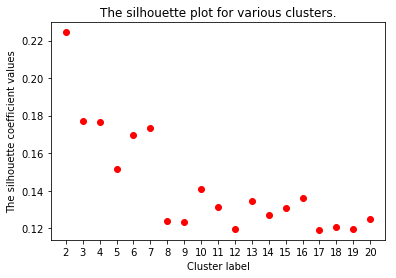
\includegraphics[width=8cm]{silhouetteall_8}
	\centering
	 \caption{Silhouette coefficient of the dataset for different number of clusters}
    \label{fig:Silhouette}
\end{figure}

\begin{figure}
	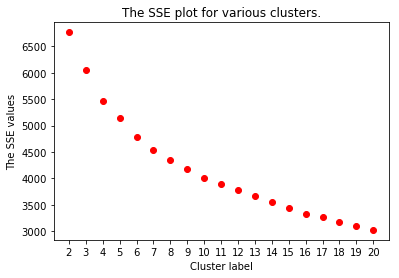
\includegraphics[width=8cm]{SSEall_8}
	\centering
	 \caption{SSE of the dataset for different number of clusters}
    \label{fig:SSE}
\end{figure}

\noindent The detail of each feature of the clustering is shown in figure \ref{fig:boxplot_cluster}. The result demonstrates a trivial contrast between the clusters; However, there are still some differentiable characteristics between the clusters:

\begin{itemize}
\item[•] The first cluster has a high level of acousticness, instrumentalness,  and tempo, whereas a low level of energy, liveness, speechiness, and loudness, suggesting that this group favors recording acoustic music with fast pace.

\item[•] The second cluster has a very high level of energy, liveness, loudness, speechiness, and valence, while the level of acoustiness, instrumentalness, and tempo remain low, implies that the user of this group might favor loud, bright live electronic music.

\item[•] The third cluster is characterized by low danceability and valence, suggesting that these users tend to listen to more negative music than other users.

\item[•] The fourth cluster has similar characteristics as the third cluster, but with higher level of acousticness and lower level of energy, suggesting that the users in this group also listen to acoustic negative music.

\item[•] The fifth cluster is characterized by low acousticness and instrumentalness. By contrast, it has high energy, loudness, tempo, and valence, suggesting that users of the group often listen to fast and happy tracks.

\item[•] The final cluster has the highest danceability and valence among the groups, implies that the users listen to dancing music. 
\end{itemize} 


\begin{figure}
  \begin{subfigure}[b]{0.3\textwidth}
    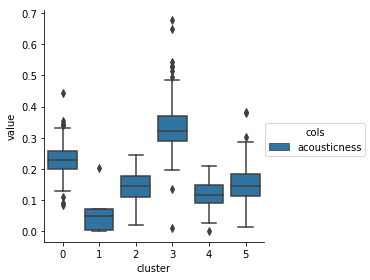
\includegraphics[width=\textwidth]{clusterting_acousticness}
    \caption{Acousticness}
    \label{fig:clusterting_acousticness}
  \end{subfigure}
  \hfill
  \begin{subfigure}[b]{0.3\textwidth}
    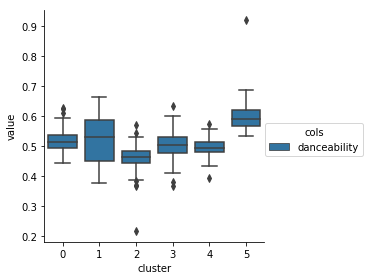
\includegraphics[width=\textwidth]{clusterting_danceability}
    \caption{Danceability}
    \label{fig:clusterting_danceability}
  \end{subfigure}
  \hfill
  \begin{subfigure}[b]{0.3\textwidth}
    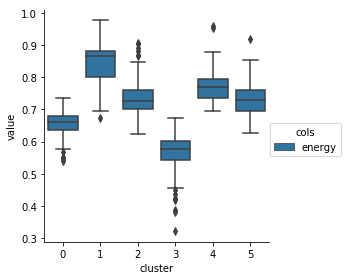
\includegraphics[width=\textwidth]{clusterting_energy}
    \caption{Energy}
    \label{fig:clusterting_energy}
  \end{subfigure}
  
  \bigskip
    \begin{subfigure}[b]{0.3\textwidth}
    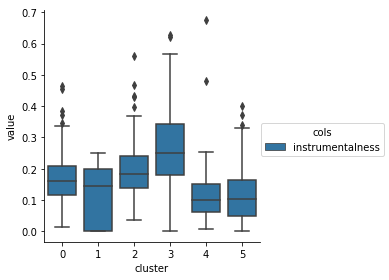
\includegraphics[width=\textwidth]{clusterting_instrumentalness}
    \caption{Instrumentalness}
    \label{fig:clusterting_instrumentalness}
  \end{subfigure}
  \hfill
    \begin{subfigure}[b]{0.3\textwidth}
    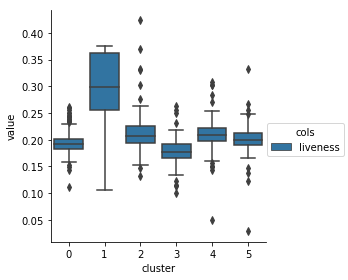
\includegraphics[width=\textwidth]{clusterting_liveness}
    \caption{Liveness}
    \label{fig:clusterting_liveness}
  \end{subfigure}
  \hfill
    \begin{subfigure}[b]{0.3\textwidth}
    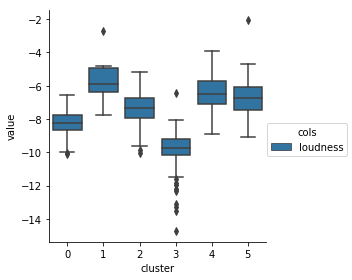
\includegraphics[width=\textwidth]{clusterting_loudness}
    \caption{Loudness}
    \label{fig:clusterting_loudness}
  \end{subfigure}
  
  \bigskip
      \begin{subfigure}[b]{0.3\textwidth}
    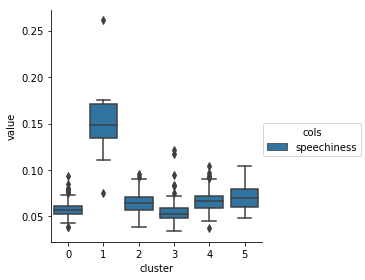
\includegraphics[width=\textwidth]{clusterting_speechiness}
    \caption{Speechiness}
    \label{fig:clusterting_speechiness}
  \end{subfigure}
  \hfill
    \begin{subfigure}[b]{0.3\textwidth}
    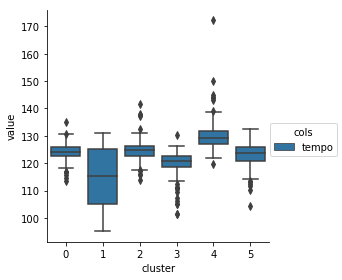
\includegraphics[width=\textwidth]{clusterting_tempo}
    \caption{Tempo}
    \label{fig:clusterting_tempo}
  \end{subfigure}
  \hfill
    \begin{subfigure}[b]{0.3\textwidth}
    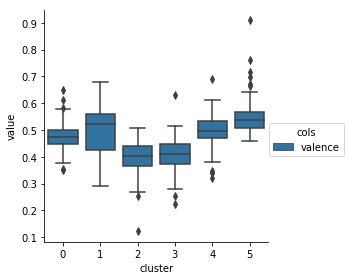
\includegraphics[width=\textwidth]{clusterting_valence}
    \caption{Valence}
    \label{fig:clusterting_valence}
  \end{subfigure}
  
  \caption{Boxplot diagram of different clusters}
  \label{fig:boxplot_cluster}
\end{figure}

\section{Experimental Setup}
The main goal of this experiment is to measure how well the learning to rank algorithm is using the described dataset, taking the two remaining algorithms as the baseline. 

\noindent The two baseline algorithms used to compare with the learning to rank algorithm is the two that were mentioned in Chapter \ref{Chapter3}. The first one is the na\"ive collaborative filtering, which is the most simple and straightforward collaborative filtering method. The second one is the matrix factorization CF for implicit feedback dataset, which is the state-of-the-art collaborative filtering. The algorithm applies two different weighting strategies: one with a constant weighting scheme, while the other uses BM25 weight scheme \cite{singhal2001modern}.

\noindent For the ranking algorithm, two versions are setup: with and without item features. For the one with item features, the features are converted from continuous to categorical values, using the following rules:

\begin{itemize}
	\item Acousticness, danceability, energy, instrumentalness, liveness, speechiness, valence: the features are divided equally into 5 bins, each has range of 0.2.
	\item Key: each key represent a category on its own.
	\item Loudness: the feature is divided equally into 12 categories, each has range of 5.
	\item Tempo: tempo is categorized using standard Italian tempo markings \cite{2018Tempo}. In details, the feature is divided into these following categories:
	\begin{itemize}
		\item Grave: tempo from 40 to 50 beat per minute (bpm).
		\item Largo: tempo from 50 to 55 bpm.
		\item Larghetto: tempo from 55 to 60 bpm.
		\item Adagio: tempo from 60 to 70 bpm.
		\item Andante: tempo from 70 to 85 bpm.
		\item Moderato: tempo from 85 to 100 bpm.
		\item Allegretto: tempo from 100 to 115 bpm.
		\item Allegro: tempo from 115 to 140 bpm.
		\item Vivace: tempo from 140 to 150 bpm.
		\item Presto: tempo from 150 to 170 bpm.
		\item Prestissimo: tempo higher than 170 bpm.
\end{itemize}	  
\end{itemize}

As there are many hyperparameters in both implicit and ranking algorithm, a sequential optimization strategy using decision trees is used to optimize the hyperparameters \cite{ForestMinimize2018}. The model is improved by sequentially evaluating the expensive function at the next best point, thereby finding the best hyperparameters with as few evaluations as possible. 

To reduce training time and approximate the best practice predicting time, instead of implementing the algorithms from scratch, I used a Python library developed by Benfred \cite{Benfred2018} for the implicit algorithm, and LightFM library \cite{DBLP:conf/recsys/Kula15} for the ranking algorithm.

\section{Score Metrics}
In this experiment, Average Precision (AP) is used to evaluate the efficiency of the algorithms. AP is defined as follow \cite{liu2009learning}:

\begin{displaymath}
AP(q) = \frac{\sum_{k=1}^m P@k(q) \cdot l_k}{\#\text{\{relevant documents\}}}
\end{displaymath}

\noindent with \( P@k \) is precision at K:

\begin{displaymath}
P@k(q) = \frac{\#\text{\{relevant documents in the top k positions\}}}{k}
\end{displaymath}

\noindent where \(m\) is the total number of document associated with query q, and \(l_k\) is the binary judgment on the relevance of the document at the \(k\)-th position. For this experiment, AP with value \(k = 1, 2, 3, 4, 5, \text{and } 10\) is measured, as we want to observe the behavior of the algorithms on optimizing for the top items. 

\section{Experiment Result}
\subsection{Accuracy}
The Average Precision of the algorithms is demonstrated in figure \ref{AP_result}. The na\"ive collaborative filtering has the poorest performance among the algorithms, with the Average Precision being 0.25 when \(k = 1\) and decreases to 0.2 when \(k = 5\), while the other two algorithms show comparable results. The learning to rank algorithm, optimizing for top items, has a slightly better precision compare to the implicit algorithm for \(k = 1 \text{ and } 2\). As \(k\) increases, the precision of all algorithms declines. The result demonstrates that adding Spotify music features does not increase the accuracy of the algorithm. 

\begin{figure}[h]
	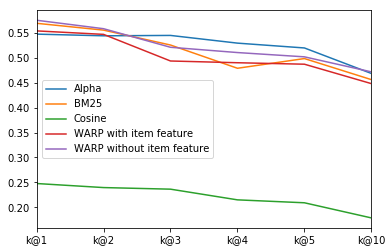
\includegraphics[width=8cm]{result}
	\centering
	\caption{Average Precision of the algorithms}
	\label{AP_result}
\end{figure}

\noindent A detail study of the behavior of each algorithms regarding different sample size is demonstrate in figure \ref{AP_with_training_size_result}. In most cases, the precision of all algorithms starts off low and builds up as the training size increases, attaining their peak accuracies as the training size grows to around 600,000, then remaining stable regardless of the continuously growing training set.

\begin{figure}[htbp]
  \begin{subfigure}[b]{0.3\textwidth}
    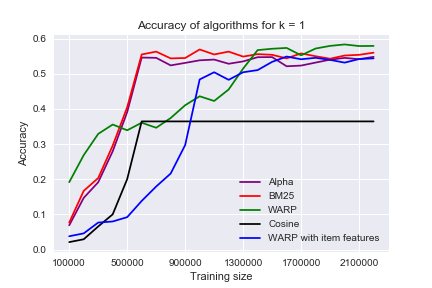
\includegraphics[width=\textwidth]{pop1}
    \caption{Average Precision of the algorithms with k = 1}
    \label{fig:pop1}
  \end{subfigure}
  \hfill
  \begin{subfigure}[b]{0.3\textwidth}
    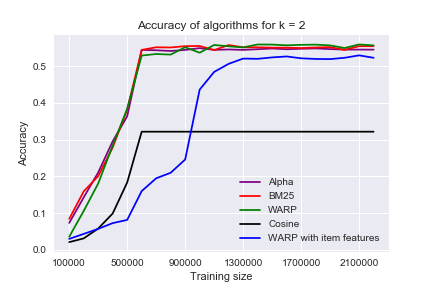
\includegraphics[width=\textwidth]{pop2}
    \caption{Average Precision of the algorithms with k = 2}
    \label{fig:pop2}
  \end{subfigure}
  \hfill
  \begin{subfigure}[b]{0.3\textwidth}
    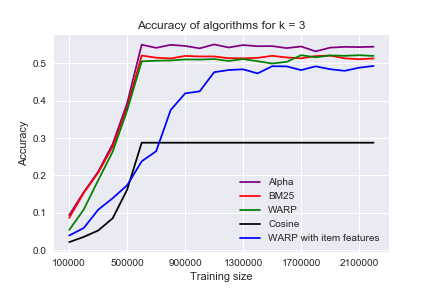
\includegraphics[width=\textwidth]{pop3}
    \caption{Average Precision of the algorithms with k = 3}
    \label{fig:pop3}
  \end{subfigure}
  
   \bigskip
    \begin{subfigure}[b]{0.3\textwidth}
    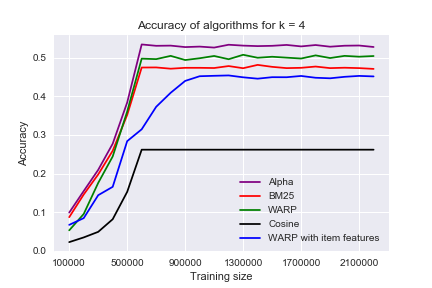
\includegraphics[width=\textwidth]{pop4}
    \caption{Average Precision of the algorithms with k = 4}
    \label{fig:pop4}
  \end{subfigure}
  \hfill
    \begin{subfigure}[b]{0.3\textwidth}
    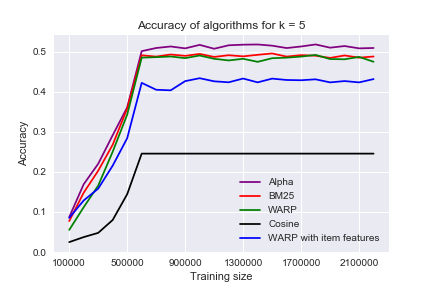
\includegraphics[width=\textwidth]{pop5}
    \caption{Average Precision of the algorithms with k = 5}
    \label{fig:pop5}
  \end{subfigure}
  \hfill
  \caption{Average Precision of the algorithms regarding training size}
  \label{AP_with_training_size_result}
\end{figure} 

\subsection{Computational expense}
Both the na\"ive collaborative filtering and the implicit collaborative filtering have linear time complexity, meaning that training time increases linearly as the number of user and item increase. The time complexity of the learning to rank algorithm, on the other hand, is \( \mathcal{O} (Y + d) \cdot D ) \), with \(Y\) is the number of classes, \(d\) is the average number of non-zero values per user array, and \(D\) is the size of the embedding space. 

\noindent A summary of the training of various algorithms is shown in figure \ref{training_time}. As the time complexity of the learning to rank algorithm is independent of the training size, training time is stable regardless of the number of entity in the dataset. Adding item features makes training time accrues as the computational complexity to optimize the rank increase; However, a careful selection of feature would shorten training time and make it invariable as training size increase. The training time of the implicit CF in this case is quite low as a result of the small size of the dataset; Nonetheless, as the size increase, training time would also linearly build up.

\begin{figure}[h]
	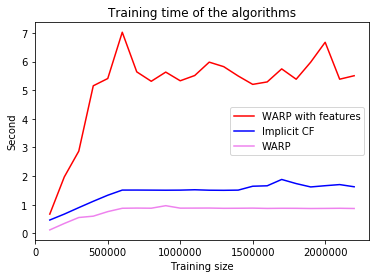
\includegraphics[width=8cm]{times_complexity}
	\centering
	\caption{Training time of the algorithms}
	\label{training_time}
\end{figure}
 

%----------------------------------------------------------------------------------------
%	THESIS CONTENT - APPENDICES
%----------------------------------------------------------------------------------------

\appendix % Cue to tell LaTeX that the following "chapters" are Appendices

% Include the appendices of the thesis as separate files from the Appendices folder
% Uncomment the lines as you write the Appendices

%% Appendix A

\chapter{Appendix A} % Main appendix title


%\include{Appendices/AppendixB}
%\include{Appendices/AppendixC}

%----------------------------------------------------------------------------------------
%	BIBLIOGRAPHY
%----------------------------------------------------------------------------------------

\printbibliography[heading=bibintoc]

%----------------------------------------------------------------------------------------

\end{document}  
